\documentclass{article}
\bibliographystyle{plain}
\linespread{1.2}
\usepackage[margin = 1.25 in]{geometry}
\usepackage{wrapfig}
\usepackage{amsfonts}
\usepackage[utf8]{inputenc}
\usepackage[T1]{fontenc}
\usepackage{graphicx}
\usepackage[english]{babel}
\usepackage[algoruled]{algorithm2e}

\renewcommand{\theequation}{\thesection.arabic{equation}}

\renewcommand{\thefigure}{\thesection.\arabic{figure}}



\renewcommand{\vec}[1]{\mathbf{#1}}
\renewcommand{\theequation}{\thesubsection.\arabic{equation}}
\DeclareGraphicsExtensions{.pdf,.png,.jpg, .gif}

\usepackage{amsthm}

\usepackage[english]{babel}
\usepackage{mathtools}

%\usepackage[OT2,T1]{fontenc}
%\DeclareSymbolFont{cyrletters}{OT2}{wncyr}{m}{n}
%\DeclareMathSymbol{\sha}{\mathalpha}{cyrletters}{"58}

\DeclareFontFamily{U}{wncy}{}
\DeclareFontShape{U}{wncy}{m}{n}{<->wncyr10}{}
\DeclareSymbolFont{mcy}{U}{wncy}{m}{n}
\DeclareMathSymbol{\Sh}{\mathord}{mcy}{"58} 
\DeclareMathOperator*{\argmin}{arg\,min}

\newcounter{eqn}
\renewcommand*{\theeqn}{\alph{eqn})}
\newcommand{\num}{\refstepcounter{eqn}\text{\theeqn}\;}

\makeatother
\newcommand{\vectornorm}[1]{\left|\left|#1\right|\right|}
\newcommand*\conjugate[1]{\bar{#1}}

\newtheorem{thm}{Theorem}
\newtheorem{defn}{Definition}
 %\theoremstyle{plain}
  \newtheorem{theorem}{Theorem}[section]
  \newtheorem{corollary}[theorem]{Corollary}
  \newtheorem{proposition}[theorem]{Proposition}
  \newtheorem{lemma}[theorem]{Lemma}
\newtheorem{example}[theorem]{Example}
  \newtheorem{definition}[theorem]{Definition}
  \newtheorem{conj}[theorem]{Conjecture}
 \newtheorem{condition}{Condition}
 \newtheorem{remark}[theorem]{Remark}

\newcommand{\supp}{\operatorname{supp}} 
\newcommand{\vc}[1]{{\mathbf{ #1}}}
\newcommand{\tn}{\widetilde{\nabla}_{n} }
\newcommand{\Z}{{\mathbb{Z}}}
\newcommand{\re}{{\mathbb{R}}}
\newcommand{\II}{{\mathbb{I}}}
\newcommand{\ep}{{\mathbb{E}}}
\newcommand{\pr}{{\mathbb{P}}}
\newcommand{\FF}{{\mathcal{F}}}
\newcommand{\TT}{{\mathcal{T}}}
\newcommand{\phin}{\phig{n}}
\newcommand{\phig}[1]{\phi^{(#1)}}
\newcommand{\ol}[1]{\overline{#1}}
\newcommand{\eff}{{\rm eff}}
\newcommand{\suc}{{\rm suc}}
\newcommand{\tends}{\rightarrow \infty}
\newcommand{\setS}{{\mathcal{S}}}
\newcommand{\setP}{{\mathcal{P}}}
\newcommand{\setX}{{\mathcal{X}}}
\newcommand{\nec}{{\rm nec}}
\newcommand{\bd}{{\rm bd}}

\title{Closed forms for distributed LASSO?}
\author{Tom Kealy}


\begin{document}

\maketitle

This is a short note (follwing \cite{Boyd2010a}), to write up some progress in seeing if the distributed ADMM version of LASSO (and also BPDN) have closed forms for their iterations.

\section{LASSO-ADMM recap}
The LASSO solves the following problem:

\begin{equation}
\argmin{x} \frac{1}{2}\|Ax-y\|_2^2 + \lambda \|x\|_1
\label{minimisation}
\end{equation}

which is put into constrained form as:

\begin{equation}
\argmin{x} \frac{1}{2}\|Ax-y\|_2^2 + \lambda \|z\|_1 \text{ s.t } x-z=0
\end{equation}

The (augmented) Lagrangian of the problem is:

\begin{equation}
L_\rho\left(x,z,\eta\right) = \frac{1}{2}\|Ax-y\|_2^2 + \lambda \|z\|_1 + \eta\left(x-z\right) + \frac{\rho}{2}\|x-z\|_2^2
\end{equation}

which in turn leads to the following set of iterations:

\begin{align}
x^{k+1} &:= \left(A^TA + \rho I\right)^{-1}\left(A^Tb +\rho\left(z^k - \eta^k\right)\right)\\
z^{k+1} &:= S_{\lambda/\rho}\left(x^{k+1} + \eta^k/\rho\right)
 \\
\eta^{k+1} &:= \eta^{k} + \rho \left(x^{k+1}-z^{k+1}\right)
\label{admm_algo_lasso}
\end{align}

Where \(S_{\lambda/\rho}\left(\circ\right)\) is the soft thresholding operator: \(S_\gamma\left(x\right)_i = sign(x_i)\left(|x_i| - \gamma\right)^+\).

\section{LASSO-ADMM on graphs}
We have a network of nodes, which individually take some measurements according to the linear system:

\begin{equation}
\vec{y} = \vec{Ax} + \vec{n}
\label{system}
\end{equation}

where \(\vec{A}\) is some measurement matrix satisfying the restricted isometry property (RIP) \cite{Candes2006}, \(\vec{y}\) are the measurements taken by the nodes, \(\vec{x}\) is the (sparse) signal we wish to reconstruct, and \(\vec{n}\) is additive white Gaussian noise. 

We model the network as an undirected graph \(G = \left(V,E\right)\), where \(V = \{1 \ldots J\}\) is the set of vertices, and \(E = V \times V\) is the set of edges. An edge between nodes \(i\) and \(j\) implies that the two nodes can communicate. The set of nodes node \(i\) can communicate with is written \(\mathcal{N}_i\) and the degree of node \(i\) is \(D_i = |\mathcal{N}_i|\). 

Individually nodes make the following measurements:

\begin{equation}
\vec{y}_p = \vec{A}_p\vec{x} + \vec{n}_p
\end{equation}

and the system \eqref{system} is formed by concatenating the individual nodes measurements together.

We assume that a proper (or approximate) colouring of the graph is available: that is each node is assigned a number from a set \(C = \{1 \ldots c \} \), and no node shares a colour with any neighbour.

To find the \(\vec{x}\) we are seeking, to each node we give a copy of \(\vec{x}, \vec{x}_p\) and we constrain the copies to be indentical across all edges in the network. 

Specifically, we are solving:

\begin{align}
\text{min}_{\bar{x} = \left(x_1, \ldots x_n\right)} \sum_J \|A_jx_j - y_j\|_2^2 + \frac{\lambda}{J}\|x\|_1
\\
\text{ and } x_i = x_j \text{ if } \{i,j\} \in E 
\label{constrainedbp}
\end{align}


The paper \cite{mota2013d} suggests that this prblem can be re-written as:

\begin{align}
\text{min}_{\bar{x} = \left(x_1, \ldots x_n\right)} \sum_J \|A_jx_j - y_j\|_2^2 + \beta\|x_j\|_1
\\
\text{ s.t. } \left(B^T \otimes I_n\right)\bar{x} = 0
\label{constrainedbp1}
\end{align}

where \(\beta = \frac{\lambda}{J}\), \( \bar{x} = \left(x_1^T, \ldots, x_J^T\right)^T \) which collects together \(J\) copies of a \(n\times 1\) vector, and \(B\) is the arc-incidence matrix: a \(V\) by \(E\) matrix where each column is associated with an edge \(\left(i,j\right) \in E\) and has \(1\) and \(-1\) in the \(ith\) and \(jth\) entry respectively. Figures \eqref{efig:ex-network} and \eqref{fig:incidence-matrix} show examples of a network and it's associated incidence matrix. Note that \(\left(B^T\otimes I_n \right) \in \re{R}^{nE \times nJ}\). 

We can also partition \(B\) and \(\bar{x}\) by colour. \( B = \left[B_1^T,\ldots , B_C^T\right]^T\),  \( \bar{x} = \left(x_1^T, \ldots, x_C^T\right)^T \). The constraints now require that \(\sum_{c=1}^C \left(B_c^T \otimes I_n\right)\bar{x}_c = 0\)

\begin{figure}[h]
\centering
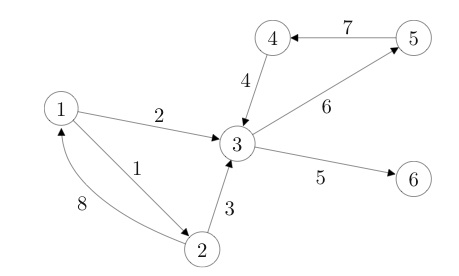
\includegraphics[height = 5 cm]{network-ex-incidence-mat.jpg}
\caption{An example of a network}
\label{efig:ex-network}
\end{figure}

\begin{figure}[h]
\centering
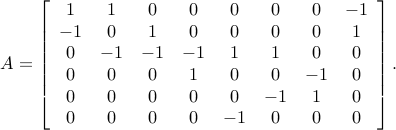
\includegraphics[height = 3 cm]{ex-incidencematrix.png}
\caption{The incidence matrix associated with \ref{efig:ex-network}}
\label{fig:incidence-matrix}
\end{figure}

The Augmented Lagrangian for the problem \eqref{constrainedbp1} can be written down as:

\begin{equation}
L = \sum_{c=1}^C \|A_jx_j - y_j\|_2^2 + \beta\|x\|_1 + \eta^T\left(B_c^T \otimes I_n\right)\bar{x}_c + \frac{\rho}{2}\|\sum_{c=1}^C \left(B_c^T \otimes I_n\right)\bar{x}_c\|^2
\end{equation}

the general update (at nodes with colour \(1\)) is:

\begin{align}
\bar{x}_1^{k+1} = \sum_{p \in C_1} \|A_px_p - y_p\|_2^2 + \beta\|x_p\|_1 + \eta^T\left(B_p^T \otimes I_n\right)\bar{x}_p + \frac{\rho}{2}\|\left(B_p^T \otimes I_n\right)\bar{x}_1 + \sum_{c=2}^C \left(B_c^T \otimes I_n\right)\bar{x}_c\|^2
\label{generic-iterations0}
\end{align}

The paper \cite[P.3]{mota2013d} shows how \eqref{generic-iterations0} can be written in the following form

\begin{align}
\bar{x}_1^{k+1} = \argmin_x \sum_{j \in C_1} \|A_1x_1 - y_1\|_2^2 + \beta\|x_1\|_1 + \left(\sum_{k \in \mathcal{N}_1} sign\left(k-1\right)\eta_{\{1,k\}} - \rho x_k \right)^T x_1 + \frac{\rho}{2}D_i\vectornorm{x_1}^2 
\label{generic-iterations}
\end{align}

where \(D_p\) is the degree of node \(p\), and \(C_1\) is the set of nodes all of the same colour. 

We should quickly note that this is an instance of the extended-ADMM algorithm:

\begin{equation*}
\begin{aligned}
& \underset{x}{\text{minimize}}
& & f_1(x_1) + f_2(x_2) + \ldots + f_q(x_q) \\
& \text{subject to}
& & U_1x_1 + U_2x_2 + \ldots U_qx_q = 0.
\end{aligned}
\end{equation*}

with \(f_r = \|A_rx_r -y_r\|_2^2 + \beta\|x_r\|^1\), \(U_r = \left(B_r^T \otimes I_n\right)\), and \(x_r\) is a local copy of \(x\) \(\forall r = 1,\ldots,C\).

The goal of this note is to introduce a set of dummy variables \(z_r\), to try to solve a problem which looks like:

\begin{equation*}
\begin{aligned}
& \underset{x}{\text{minimize}}
& & g_1(x_1) + h_1(z_1)  + \ldots + g_q(x_q) + h_q(x_2) \\
& \text{subject to}
& & U_1x_1 + V_1z_1 \ldots U_qx_q + V_qz_q = 0.
\end{aligned}
\end{equation*}

with \(g_r = \|A_rx_r -y_r\|_2^2\), \(h_r = \beta\|x_r\|^1\), \(U_r = \left(B_r^T \otimes I_n\right)\), \(V_r = -I\) and \(x_r, z_r\) are a local copies of \(x,z\) \(\forall r = 1,\ldots,C\). We seek a set of closed form iterations for the minimisation \eqref{generic-iterations}, as \eqref{generic-iterations} cannot be done without an auxiliary minimisation algorithm.

The re-writing hinges on re-writing the the second and third terms of \eqref{generic-iterations0}. 

The third term can be written as:

\begin{align*}
&\frac{\rho}{2}\|\left(B_1^T \otimes I_n\right)\bar{x}_1 + \sum_{c=2}^C \left(B_1^T \otimes I_n\right)\bar{x}_j\|^2 = \\
& \frac{\rho}{2}\bar{x}_1^T  \left(B_1^T \otimes I_n\right)^T \left(B_1^T \otimes I_n\right) \bar{x}_1 + \rho \bar{x}_1^T \sum	_{c=2}^C \left(B_1^T \otimes I_n\right)^T \left(B_c^T \otimes I_n\right) \bar{x}_c + \|\sum_{c=2}^C  \left(B_c^T \otimes I_n\right) \bar{x}_c\|^2
\end{align*}

We will investigate the first and second terms more, as the last term doesn't depend on \(\bar{x}_1\) and can be dropped.

\begin{lemma}
\begin{equation}
\frac{\rho}{2}\bar{x}_1^T  \left(B_1^T \otimes I_n\right)^T \left(B_1^T \otimes I_n\right) \bar{x}_1 = \frac{\rho}{2}\sum_{l \in C_1} D_l \|x_l\|^2
\end{equation}

\begin{proof}
\(\left(B_1^T \otimes I_n\right)^T \left(B_1^T \otimes  I_n\right) = B_1B_1^T \otimes I_n\) from taking the transpose of the first term, and using the properties of the Kronecker product. \(BB^T\) is a \(J \times J\) matrix, with the degree of the nodes on the main diagonal and \(-1\) in position \(\left(i,j\right)\) if nodes \(i\) and \(j\) are neighbours (i.e \(BB^T\) is the graph Laplacian). The trace of \(B_1B_1^T\) is simply the sum of the degrees of nodes with colour 1. 
\end{proof}
\label{diagonallemma}
\end{lemma}

\begin{lemma}
\(\rho \bar{x}_1^T \sum	_{c=2}^C \left(B_1^T \otimes I_n\right)^T \left(B_c^T \otimes I_n\right) \bar{x}_c = -\rho\sum_{l\in C_1} \sum_{m\in N_l} x_l^Tx_m^k\)
\begin{proof}
\(\left(B_1^T \otimes I_n\right)^T \left(B_c^T \otimes  I_n\right) = B_1B_c^T \otimes I_n\) by repeating the steps from lemma \ref{diagonallemma}.  \(B_1B_c^T\) corresponds to an off diagonal block of the graph Laplacian, and so counts how many neighbours each node with colour 1 has.
\end{proof}
\label{lem:cross-terms}
\end{lemma}

Finally, we need to consider the second term from \eqref{generic-iterations0}:

\begin{equation}
\eta^T\left(B_1^T \otimes I_n\right)\bar{x}_1 = \sum_{l\in C_1} \sum_{m\in N_l}sign\left(m-l\right)\eta_{ml}^T x_l
\label{eq:graph-multiplier}
\end{equation}

where \(\eta\) is decomposed edge-wise: \(\eta = \left(\ldots, \eta_{ij},\ldots\right)\), such that \(\eta_{i,j} = \eta_{j,i}\) and is associated with the constraint \(x_i = x_j\).

adding together this with the two lemmas, lets us write \eqref{generic-iterations0} as \eqref{generic-iterations}.

To tidy \eqref{generic-iterations} up define:

\begin{equation}
\nu_i = \left(\sum_{k \in \mathcal{N}_i} sign\left(k-i\right)\eta_{\{i,k\}} - \rho x_k \right)
\end{equation}

this is a rescaled version of the Lagrange multiplier, \(\eta\), which respects the graph structure. Finally \eqref{generic-iterations0} reduces to:

\begin{align}
\bar{x}_1^{k+1} = \sum_{j \in C_1} \|A_1x_1 - y_1\|_2^2 + \|x_1\|_1 + \nu_1^T x_1 + \frac{\rho}{2}D_i\vectornorm{x_1}^2
\label{generic-iterations-nice}
\end{align}

We seek a set of closed form iterates, like \eqref{admm_algo_lasso} except now including information about the network.

To this end we can write \eqref{constrainedbp1} as:

\begin{align}
\text{min}_{\bar{x} = \left(x_1, \ldots x_n\right)} \sum_J \|A_jx_j - y_j\|_2^2 + \|z_j\|_1
\\
\text{ s.t. } \left(B^T \otimes I_n\right)\bar{x} = 0
\\
\text{ and } \bar{x} - \bar{z} = 0
\label{constrainedbp2:switching trick}
\end{align}

which can be written more compactly as:

\begin{align}
\text{min}_{\bar{x} = \left(x_1, \ldots x_n\right)} \sum_J \|A_jx_j - y_j\|_2^2 + \|z_j\|_1
\\
\text{ s.t. } \left(\left(B^T \otimes I_n\right) + I_n \right)\bar{x} - \bar{z} = 0
\label{constrainedbp2:switching trick}
\end{align}

The Augmented Lagrangian for this problem can be written down as:

\begin{equation}
L = \sum_J \|A_jx_j - y_j\|_2^2 + \|x_j\|_1 + \eta^T M \bar{x} - \bar{z} + \frac{\rho}{2}\|M\bar{x} - \bar{z}\|^2
\end{equation}

where we have defined \(M = \left(\left(B^T \otimes I_n\right) + I_n \right) \)

\textbf{Conjecture}:

Following steps similar to \cite{mota2013d} this Lagrangian can be written in the following form 

\begin{equation}
L = \sum_J \|A_jx_j - y_j\|_2^2 + \|z_j\|_1 + \nu_j^T \left(x_j-z_j\right) + \frac{\rho}{2}D_i\vectornorm{x_j-z_j}^2
\end{equation}

Then by differentiating with respect to \(x_j\) and \(z_j\) we  can find closed forms for the updates as:

\begin{align}
x_j^{k+1} &:= \left(A_j^TA_j + \rho D_J I\right)^{-1}\left(A_j^Ty_j +\rho D_j z^k - \nu^k\right)\\
z^{k+1} &:= S_{\lambda/J}\left(x_j^{k+1} + \frac{1}{\rho D_j}\nu_j^{k+1}\right)
 \\
\nu^{k+1} &:= \nu^{k} + \rho \left(x^{k+1}-z^{k+1}\right)
\label{dadmm_algo_lasso}
\end{align}

As a step towards this, we need to work out what \(\bar{x}_1^T  M_1^T M_1 \bar{x}_1\) and \(\bar{x}_1^T\sum_{c=2}^C M_1^TM_c\bar{x}_c\) is in our case.

\begin{align*}
&\bar{x}_1^T\left(\left(B^T \otimes I_n\right) + I_n \right)^T\left(\left(B^T \otimes I_n\right) + I_n \right)\bar{x}_1 = \\& \bar{x}_1\left(B_1B_1^T \otimes I_n + I_n^T\left(B_1^T \otimes I_n\right)
+ \left(B_1^T \otimes I_n\right)^TI_n + I_n\right)\bar{x}_1
\end{align*}

we know what \(\bar{x}_1^T\left(B_1B_1^T \otimes I_n\right)\bar{x}_1\) is, from lemma \ref{diagonallemma}. The second and third terms \(\bar{x}_1^T\left(B_1^T \otimes I_n\right)\bar{x}_1\) and \(\bar{x}_1^T\left(B_1^T \otimes I_n\right)^T\bar{x}_1\) will equal zero because \(\left(B_1^T \otimes I_n\right)\bar{x}_1 = 0 \) from the constraints of the problem.

Also,

\begin{align*}
&\rho \bar{x}_1^T \sum_{c=2}^C \left(\left( B_1^T \otimes I_n\right)+I_n\right)^T \left(\left( B_c^T \otimes I_n\right)+I_n\right) \bar{x}_c = \\ &\rho\bar{x}_1^T\sum_{c=1}^C\left( \left(B_1B_c^T \otimes I_n\right) + \left(B_c^T \otimes I_n\right)I_n^T
+ I_n\left(B_1^T \otimes I_n\right)^T + I_n\right)\bar{x}_c
\\
&= -\rho\sum_{l\in C_1} \sum_{m\in N_l} x_l^Tx_m^k + \rho\sum_{c=2}^C\bar{x}_1^T\bar{x}_c
\end{align*}

using lemma \ref{lem:cross-terms}, and again the middle terms are equal to \(0\). 

The final term to deal with is:

\begin{equation}
\eta^T\left(\left(B_1^T \otimes I_n\right)+I_*\right) = \eta^T\left(B_1^T \otimes I_n\right)\bar{x}_1 + \eta^TI_8\bar{x}_1
\end{equation}

the first term we have dealt with previously in \eqref{eq:graph-multiplier}.

Collecting all terms together we now have:

\begin{align}
&\eta^T\left(\left(B_1^T \otimes I_n\right)+I_*\right) + \|\sum	_{c=1}^C M_c\bar{x}_c\|^2 = \\
&\eta^T\left(B_1^T \otimes I_n\right)\bar{x}_1 + \eta^TI_8\bar{x}_1 + -\rho\sum_{l\in C_1} \sum_{m\in N_l} x_l^Tx_m^k + \rho\sum_{c=2}^C\bar{x}_1^T\bar{x}_c +  B_1B_1^T \otimes I_n + \|x_1\|^2
\end{align}

so, collecting all terms together we have:

\begin{equation}
L =\sum{l\in c_1} \|A_lx_l - y_l\|_2^2 + \beta\|z_l\|_1  + \nu_l^T\bar{x}_1 + \frac{\rho D_l}{2}\|x_l\|^2 + \|x_l\|^2 + \rho\sum_{c=2}^Cx_l^Tx_c + \eta^TI_*
\end{equation}

collecting like terms together we have:

\begin{equation}
L = \sum{l\in c_1} \|A_lx_l - y_l\|_2^2 + \beta\|z_l\|_1 + \mu^T\bar{x}_l + \gamma\|x_l\|^2
\end{equation}

where

\begin{equation}
\mu = \sum_{m \in N_l}\left(sign\left(m-l\right)+1\right)\eta^T - 2\rho\bar{x}_m
\end{equation}

and 

\begin{equation}
\gamma = 1+ \frac{\rho D_l}{2}
\end{equation}

\section{Second Attempt}

Define

\begin{equation}
v := \left(\left(B^T \otimes I_n\right)+I\right)\bar{x}-\bar{z} = \sum_{j=1}^J \left[\left(B^Te_j\right)\otimes x_j - e_j\otimes z_j\right]
\end{equation}

where we have defined \(\bar{x} = \sum_{j=1}^J e_j \otimes x_j\) and \(e_j\) is a \(J \times 1\) unit vector.

we are trying to calculate \(v^Tv\). 

\begin{align*}
v^Tv &= \sum_{k=1}^J \sum_{j=1}^J \left[\left(e_k^TB\right)\otimes x_k^T - e_k^T\otimes z_k\right] \left[\left(B^Tw_c\right)\otimes \bar{x}_j - e_j\otimes z_j\right] \\
&= \sum_{k,j} \left(e_k^TBB^Te_j \otimes x_k^Tx_j\right) - \left(e_k^TBe_j \otimes x_k^Tz_j\right) - \left(e_k^T B^Te_j \otimes z_k^T x_j\right) + \left(e_k^T e_j \otimes z_k^T z_j\right)
\end{align*}

Now \(\left(e_k^T B^Te_j \otimes z_k^T x_j\right) = 0\) as the first term \( e_k^T B^Te_j  \) is an inner product between a \(J\times 1\)vector containing a single \(1\) and a single \(-1\) and a \(1\times J\) vector containing all \(1s\). Similar reasoning applies to the other cross term.

So:

\begin{align*}
v^Tv &= \sum_{k,j} \left(e_k^TBB^Te_j \otimes x_k^Tx_j\right) + \left(e_k^T e_j \otimes z_k^T z_j\right)
\end{align*}

we can try to solve the same problem with a smaller parameter space: write \(c\left(i\right)\) for the colour of the \(i^{th}\) node, and \(w_c\) for the vector identifying the nodes of colour \(c\). Then we can equivalently write 

\begin{equation}
\bar{x} = \sum_{c=1}^C w_c \otimes x_c
\end{equation}

as before, define

\begin{equation}
v := v := \left(\left(B^T \otimes I_n\right)+I\right)\bar{x} - \bar{z} = \sum_{c=1}^C \left[\left(B^Tw_c\right)\otimes x_c - w_c\otimes z_c\right]
\end{equation}

\begin{align*}
v^Tv &= \sum_{e=1}^C \sum_{c=1}^C \left[\left(w_e^TB\right)\otimes x_e^T - w_e^T\otimes z_e^T\right]  \left[\left(B^Tw_c\right)\otimes x_c - w_c\otimes z_c\right] \\
&= \sum_{e,c} \left(w_e^TBB^Tw_c \otimes x_e^Tx_c\right) - \left(w_e^TBw_c \otimes x_e^Tz_c\right) - \left(w_e^T B^Tw_c \otimes z_e^T x_c\right) + \left(w_e^T w_c \otimes z_e^T z_c\right)
\end{align*}

\section{Third Attempt}

Earlier today (\today), we wrote down two Lagrangians as there was some confusion (on my end) about which one would be preferable. They were:

\begin{equation}
L = \sum_{colours} \|A_jx_j - y_j\|_2^2 + \|z_j\|_1 + \eta^T M \bar{x} +\theta^T\left(\bar{x} - \bar{z}\right) + \frac{\rho}{2}\|M\bar{x} + \bar{x} - \bar{z}\|^2
\end{equation} 

where \(M = \left(B^T \otimes I_n\right)\), and 

\begin{equation}
L = \sum_{colours} \|A_jx_j - y_j\|_2^2 + \|z_j\|_1 + \eta^T M \bar{x} +\theta^T\left(\bar{x} - \bar{z}\right) + \frac{\rho}{2}\|M\bar{x}\|^2 + \frac{\rho}{2}\|\bar{x} - \bar{z}\|^2
\label{correctL}
\end{equation} 

The second \eqref{correctL} Lagrangian is correct, as \(Mx+(x-z)\) isn't legal. This is fortuitous, as we can use the heavy lifting from \cite{mota2013d} to write the Lagrangian as:

\begin{equation}
L = \sum_{colours} \|A_jx_j - y_j\|_2^2 + \|z_j\|_1 + \nu^T \bar{x} +\theta^T\left(\bar{x} - \bar{z}\right) + \frac{\rho D_j}{2}\|\bar{x}_j\|^2 + \frac{\rho}{2}\|\bar{x}_j - \bar{z}_j\|^2
\end{equation}

which is definitely differentiable, re \(x,z,\nu,theta\).



\bibliography{cswireless1}

\end{document}